\documentclass[a4paper,12pt]{report}

% Pacotes necessários
\usepackage[utf8]{inputenc}
\usepackage[brazil]{babel}
\usepackage{hyperref}
\usepackage[T1]{fontenc}
\usepackage{graphicx}
\usepackage{caption}
\usepackage[left=2.5cm, right=2.5cm, top=2.5cm, bottom=2.5cm]{geometry}
\usepackage{float}
\usepackage{amsmath}
\usepackage{amsfonts}
\usepackage{amssymb}
\usepackage{listings}
\usepackage{xcolor}
\usepackage{booktabs}
\usepackage{siunitx}
\usepackage{subcaption}
\usepackage{enumitem}
\usepackage{titlesec}
\usepackage{fancyhdr}

% Configuração de cabeçalhos
\pagestyle{fancy}
\fancyhf{}
\fancyhead[L]{Sistemas de Controle - Reator Químico}
\fancyhead[R]{UFSC - EEL}
\fancyfoot[C]{\thepage}

% Configuração de seções
\titleformat{\chapter}{\huge\bfseries}{\thechapter}{20pt}{\Huge}
\titleformat{\section}{\Large\bfseries}{\thesection}{1em}{}
\titleformat{\subsection}{\large\bfseries}{\thesubsection}{1em}{}
\titleformat{\subsubsection}{\normalsize\bfseries}{\thesubsubsection}{1em}{}

% Configuração de listings
\lstset{
    language=Matlab,
    basicstyle=\ttfamily\footnotesize,
    keywordstyle=\color{blue}\bfseries,
    commentstyle=\color{green!60!black},
    stringstyle=\color{red},
    showstringspaces=false,
    breaklines=true,
    frame=single,
    numbers=left,
    numberstyle=\tiny\color{gray},
    backgroundcolor=\color{gray!10},
    tabsize=2,
    captionpos=b
}

% Configuração da página de título
\newcommand{\reporttitle}{Análise e Projeto de Sistemas de Controle para Reator Químico Continuamente Agitado}
\newcommand{\reportsubtitle}{Estudo Comparativo de Técnicas de Controle com Aplicação em Processo Industrial}
\newcommand{\reportauthor}{Lucas William Junges}
\newcommand{\reportdate}{\today}
\newcommand{\reportinstitution}{Universidade Federal de Santa Catarina}
\newcommand{\reportdepartment}{Departamento de Engenharia Elétrica e Eletrônica}
\newcommand{\reportcourse}{Sistemas de Controle}

\begin{document}

% Página de título personalizada
\begin{titlepage}
    \centering
    \vspace*{1cm}
    
\includegraphics[width=0.3\textwidth]{Imagens/BrasaoUFSC.png}
    \par\vspace{1cm}
    {\scshape\Large \reportinstitution\par}
    {\scshape\normalsize \reportdepartment\par}
    \vspace{1.5cm}
    {\huge\bfseries \reporttitle\par}
    \vspace{0.5cm}
    {\Large\itshape \reportsubtitle\par}
    \vspace{2cm}
    {\Large\textbf{Autor:}\par}
    {\Large \reportauthor\par}
    \vspace{1.5cm}
    {\large\textbf{Disciplina:} \reportcourse\par}
    \vspace{1cm}
    \vfill
    {\large \reportdate\par}
\end{titlepage}

\tableofcontents
\listoffigures
\clearpage

\chapter{Introdução}
Este relatório apresenta um estudo abrangente sobre o projeto e análise de sistemas de controle aplicados a um reator químico continuamente agitado (CSTR) utilizado na produção industrial de cyclopentenol. O trabalho está estruturado em três partes principais que abordam progressivamente técnicas de controle de crescente complexidade e sofisticação.

A primeira parte concentra-se na análise fundamental do sistema, incluindo a caracterização do comportamento estático e dinâmico do reator, linearização em torno de um ponto de operação, e o projeto de um controlador PI básico utilizando a técnica de alocação de polos. A segunda parte avança para o projeto de controladores por lugar das raízes, explorando estratégias de controle em malha simples e múltipla, incluindo controle feedforward. A terceira parte aborda o desafio de controle na presença de atrasos de medição, implementando a técnica do Preditor de Smith.

O sistema estudado representa um processo típico da indústria química, onde a concentração do produto B (cyclopentenol) deve ser controlada através da manipulação da vazão de diluição, na presença de perturbações na concentração de alimentação.

\chapter{Parte I: Análise e Controle por Alocação de Polos}
\section{Análise do Sistema em Equilíbrio}
A dinâmica do processo é regida por:
\[ A \xrightarrow{k_1} B \xrightarrow{k_2} C \]
\[ 2A \xrightarrow{k_3} D\]
\begin{align}
\frac{dC_a(t)}{dt} &= -k_1 C_a(t) - k_3 C_a(t)^2 + \frac{(C_{af}(t) - C_a(t)) F(t)}{V} \\
\frac{dC_b(t)}{dt} &= k_1 C_a(t) - k_2 C_b(t) - \frac{C_b(t) F(t)}{V}
\end{align}
Com \(u = F/V\), as equações de equilíbrio (\(\frac{dC}{dt} = 0\)) são:
\begin{align}
C_{a_f} u &= C_a^2 k_3 + C_a (k_1 + u) \\
C_a k_1 &= C_b(k_2 + u)
\end{align}
A análise dessas equações no MATLAB para a faixa de operação de \(u\) e \(C_{af}\) gera os mapas de comportamento estático.

% Figura temporariamente comentada para debugging de compilação
% \begin{figure}[H]
%     \centering
%     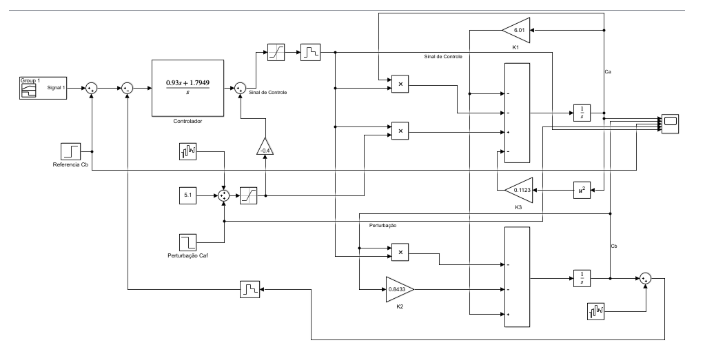
\includegraphics[width=0.7\textwidth]{"Trabalho 2 Sistemas de Controle/image1.png"}
%     \caption{Comparação de desempenho: Controlador PI (azul) vs. Controlador por LR (vermelho).}
% \end{figure}
\textit{(Figura temporariamente removida para fins de compilação. Será reinserida após resolução do problema.)}

\section{Linearização e Projeto do Controlador PI}
Para o ponto de operação \( C_{af} = 5.1 \) mol/L e \( u = 1 \) min\(^{-1}\), as concentrações de equilíbrio são \( \overline{C}_a = 0.719 \) e \( \overline{C}_b = 2.345 \) mol/L. O modelo linearizado em torno deste ponto é:
\begin{align}
\Delta\frac{dC_a}{dt} &= -7.171 \Delta C_a + \Delta C_{a_f} + 4.381\Delta u \\
\Delta\frac{dC_b}{dt} &= 6.01 \Delta C_a -1.843\Delta C_b - 2.354 \Delta u
\end{align}
Com base neste modelo, um controlador PI \(C(s)\) e um filtro de referência \(F_r(s)\) foram projetados por alocação de polos para atender \(t_{5\%} \in [1.5, 1.7]\) min e pico \(< 5\%\).
\begin{align}
C(s) &= 1.85162 \frac{s + 1.91627}{s} \\
F_r(s) &= \frac{1.91627}{s + 1.91627}
\end{align}
A simulação do sistema não linear com o controlador projetado mostra que as especificações são atendidas perto do ponto de operação, mas o desempenho degrada ao se afastar dele.

% Figura temporariamente comentada para debugging de compilação
% \begin{figure}[H]
%     \centering
%     \includegraphics[width=0.8\linewidth]{{"Trabalho 1 Sistemas de Controle/respostacompequenasvariaçoes"}.png}
%     \caption{Resposta do sistema não linear com controlador para pequenas variações.}
% \end{figure}
\textit{(Figura temporariamente removida para fins de compilação. Será reinserida após resolução do problema.)}

\chapter{Parte II: Controle por Lugar das Raízes e Feedforward}
\section{Projeto de Controle por Lugar das Raízes (LR)}
Nesta parte, um controlador mais complexo é projetado usando a técnica do Lugar das Raízes para o modelo de segunda ordem. A função de transferência de interesse é:
\begin{equation}
\frac{ C_b(s)}{u(s)} = \frac{-2.354(s-4.013)}{(s + 1.843)(s + 7.171)}
\end{equation}
O controlador projetado, que tem uma estrutura PID, é:
\begin{equation}
C(s)=\frac{5.2946(s+3.835)^2}{s(s+20)}  
\end{equation}
Este controlador, quando comparado ao PI da Parte I, oferece uma resposta mais suave e menos oscilatória, sendo mais adequado para a dinâmica de segunda ordem do sistema.

% Figura temporariamente comentada para debugging de compilação
% \begin{figure}[H]
%     \centering
%     \includegraphics[width=0.7\textwidth]{"Trabalho 2 Sistemas de Controle/image1".png}
%     \caption{Comparação de desempenho: Controlador PI (azul) vs. Controlador por LR (vermelho).}
% \end{figure}
\textit{(Figura temporariamente removida para fins de compilação. Será reinserida após resolução do problema.)}

\section{Melhora com Controle Feedforward}
Para melhorar a rejeição à perturbação \(C_{af}\), uma estratégia de controle Feedforward é implementada. O controlador feedforward ideal é instável, então uma aproximação por ganho estático é utilizada:
\begin{equation}
C_{ff} \approx -0.4
\end{equation}
A simulação mostra uma melhoria drástica na rejeição à perturbação.

% Figura temporariamente removida para debugging de compilação
% \begin{figure}[H]
%      \centering
%      \begin{subfigure}[b]{0.48\textwidth}
%          \centering
%          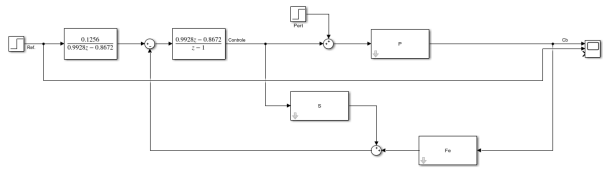
\includegraphics[width=\textwidth]{"Trabalho 2 Sistemas de Controle/image3.png"}
%          \caption{Sem Feedforward}
%          \label{fig:sem_ff}
%      \end{subfigure}
%      \hfill
%      \begin{subfigure}[b]{0.48\textwidth}
%          \centering
%          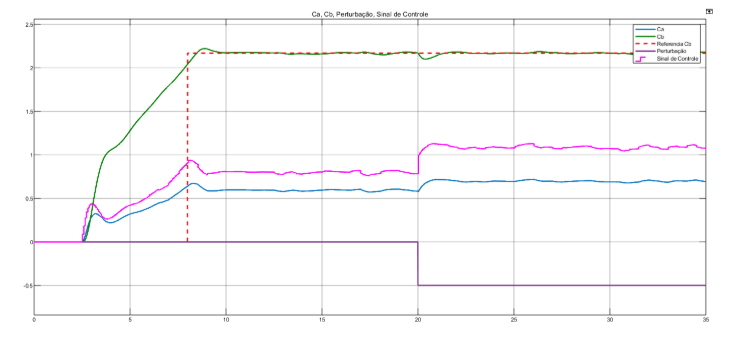
\includegraphics[width=\textwidth]{"Trabalho 2 Sistemas de Controle/image2.png"}
%          \caption{Com Feedforward}
%          \label{fig:com_ff}
%      \end{subfigure}
%      \caption{Comparação da rejeição à perturbação com e sem controle Feedforward.}
% \end{figure}
\textit{(Figura temporariamente removida para fins de compilação. Será reinserida após resolução do problema.)}

\chapter{Parte III: Controle com Atraso de Medição}
\section{O Desafio do Atraso de Tempo}
Esta seção aborda um cenário mais realista onde a medição da concentração \(C_b\) possui um atraso de transporte de 3 minutos. Este atraso, modelado como \(e^{-3s}\), degrada severamente o desempenho de controladores convencionais.

\section{Solução: Preditor de Smith}
A estrutura do Preditor de Smith é utilizada para compensar o atraso. Ela funciona utilizando um modelo matemático do processo para "prever" a saída futura, removendo o efeito do atraso da malha de realimentação. Isso permite que o controlador principal, projetado para o processo sem atraso, opere de forma eficaz.

% Figura temporariamente comentada para debugging de compilação
% \begin{figure}[H]
%     \centering
%     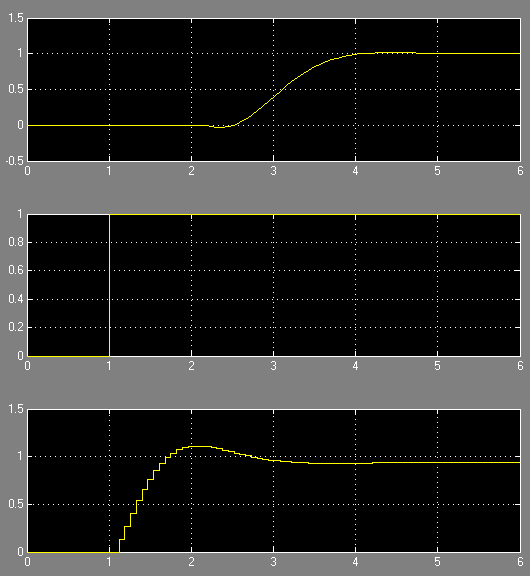
\includegraphics[width=0.7\textwidth]{Imagens/q13.png}
%     \caption{Estrutura conceitual do Preditor de Smith.}
%     \label{fig:smith_predictor}
% \end{figure}
\textit{(Figura temporariamente removida para fins de compilação. Será reinserida após resolução do problema.)}

O controlador \(C(s)\) é o mesmo projetado na Parte II. O bloco \(G_p(s)\) é o modelo do processo sem atraso, e \(e^{-Ls}\) é o modelo do atraso. A diferença entre a saída real do processo e a saída do modelo (\(\epsilon\)) corrige erros de modelagem.

\subsection{Resultados da Simulação}
A simulação do sistema com o Preditor de Smith mostra que o desempenho desejado (tempo de acomodação e sobressinal) é recuperado, apesar do grande atraso. A análise de robustez, no entanto, mostra que o desempenho é sensível a erros na estimativa do atraso. Uma variante, o Preditor de Smith filtrado, pode ser usada para melhorar a robustez, ao custo de uma maior complexidade.

\chapter{Conclusões Gerais}
Este trabalho demonstrou a aplicação progressiva de técnicas de controle a um reator químico.
\begin{itemize}
    \item \textbf{Parte I (PI):} Solução simples e robusta, adequada para controle básico, mas com desempenho limitado para dinâmicas complexas.
    \item \textbf{Parte II (LR + FF):} Oferece desempenho superior, com resposta mais suave e excelente rejeição a perturbações, mas exige um projeto mais complexo e sensores adicionais.
    \item \textbf{Parte III (Preditor de Smith):} Essencial para processos com atrasos significativos, restaurando o desempenho do controle, mas sensível a erros de modelagem.
\end{itemize}
A escolha da estratégia de controle em um cenário industrial dependerá de um trade-off entre o desempenho desejado, a complexidade da implementação e os custos associados (sensores, poder computacional).

\begin{thebibliography}{9}
    \bibitem{ogata} Ogata, K. \textit{Engenharia de Controle Moderno}. 5ª edição. Pearson Prentice Hall, 2010.
    \bibitem{dorf} Dorf, R. C.; Bishop, R. H. \textit{Sistemas de Controle Modernos}. 12ª edição. LTC, 2013.
    \bibitem{seborg} Seborg, D. E.; Edgar, T. F.; Mellichamp, D. A. \textit{Process Dynamics and Control}. 3ª edição. Wiley, 2010.
\end{thebibliography}

\end{document}
